%! Author = Filippo Vissani
%! Date = 08/02/24
% !TeX root = ../thesis-main.tex

%----------------------------------------------------------------------------------------
\chapter{Evaluation}
\label{chap:evaluation}
%----------------------------------------------------------------------------------------

Validation is the process within software development, encompassing measures to guarantee that the software aligns with predefined requirements and specifications, and is suitable for its designated purpose. This crucial step ensures that the software operates without flaws, meets user expectations, and executes its intended functions accurately. The validation process entails a range of testing methodologies, each aimed at verifying that the software achieves its objectives and behaves as anticipated across diverse environments and scenarios.

\section{Testing}

To ensure the accuracy of the code developed, the project implemented a comprehensive suite of unit tests to validate the implementation. This approach not only instilled confidence in refactoring efforts but also formalized expectations regarding the language's API, enabling verification and reproducibility. Specifically, unit tests were crafted using Kotest\footnote{\url{https://kotest.io/}} framework, a widely accepted tool for automated testing in Kotlin. Among its testing styles, the project opted for \texttt{StringSpec} due to its straightforward structure, which facilitates a behavior-driven approach to test composition.

\lstinputlisting[float,language=kotlin,label={lst:rexchange-test},caption=TODO.]{listings/rexchange-test.kt}

\section{Analysis of the Ergonomics of the Proposed Models}

\begin{figure}
    \centering
    \begin{subfigure}[b]{.15\textwidth}
        \centering
        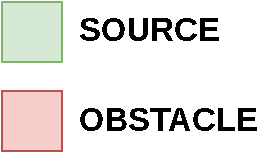
\includegraphics[width=\textwidth]{figures/gradient-environment-legend.pdf}
        \label{fig:gradient-legend}
    \end{subfigure}
    \hfill
    \begin{subfigure}[b]{.49\textwidth}
        \centering
        
\includegraphics[width=\textwidth]{figures/palette-cropped2.png}
        \label{fig:gradient-palette}
    \end{subfigure}
    \hfill
    \begin{subfigure}[b]{.49\textwidth}
        \centering
        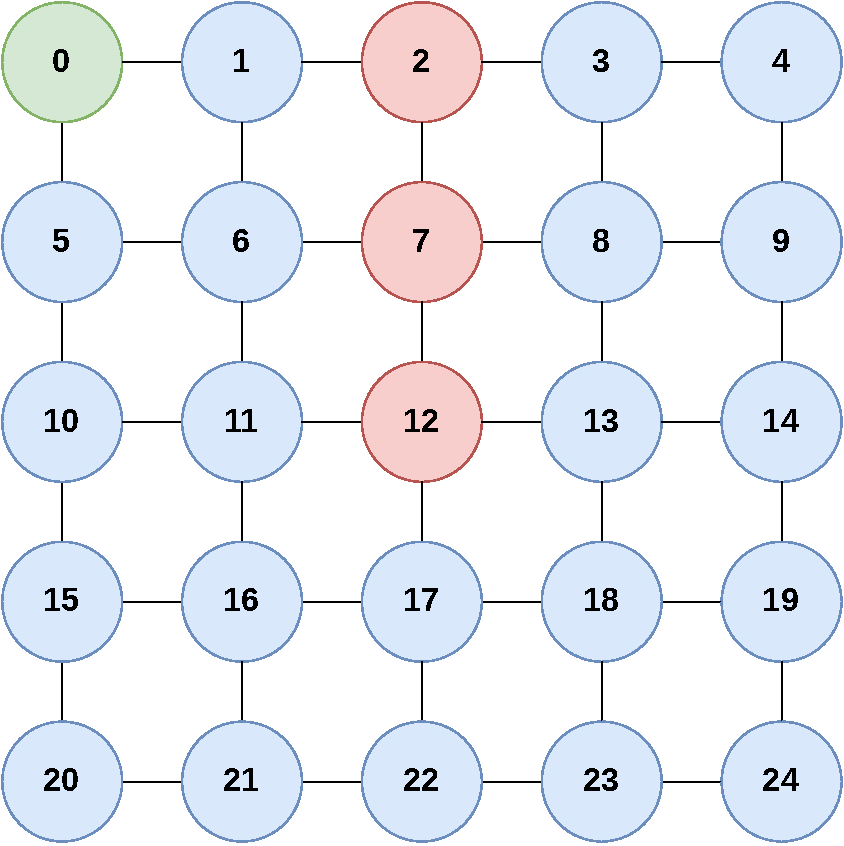
\includegraphics[width=\textwidth]{figures/gradient-environment.pdf}
        \caption{TODO.}
        \label{fig:gradient-envronment}
    \end{subfigure}
    \hfill
    \begin{subfigure}[b]{.49\textwidth}
        \centering
        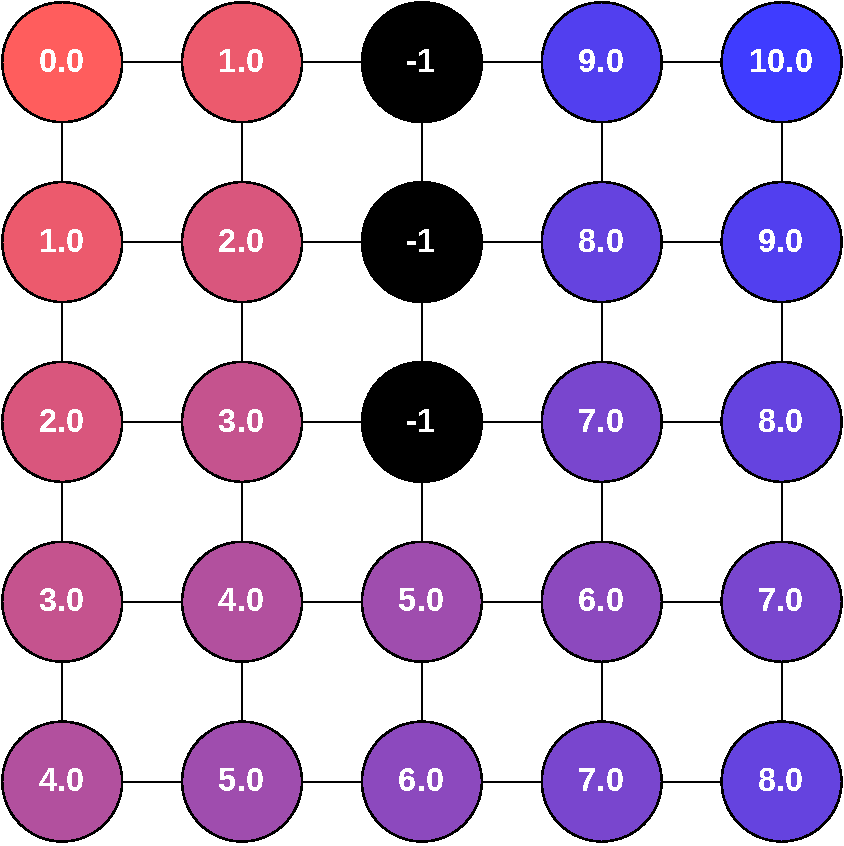
\includegraphics[width=\textwidth]{figures/gradient-environment-execution.pdf}
        \caption{TODO.}
        \label{fig:gradient-envronment-execution}
    \end{subfigure}
\end{figure}

\lstinputlisting[float,language=kotlin,label={lst:simulation-configuration},caption=TODO.]{listings/simulation-configuration.kt}

\subsection{Purely Reactive Model}

\lstinputlisting[float,language=kotlin,label={lst:gradient-obstacles-prm},caption=TODO.]{listings/gradient-obstacles-prm.kt}

\subsection{Model with Reactive Messages and Sensors}

\lstinputlisting[float,language=kotlin,label={lst:gradient-obstacles-rmsm},caption=TODO.]{listings/gradient-obstacles-rmsm.kt}
